In this section we discuss two core buliding block classes: (1) {\cbalgo} and (2) {\cbkeeper}. Though we discuss these basic {\CPP} classes first, it might be easier to understand these classes after you read about {\cmerge}, described in Sec.{\ref{sec:fmwk:cmerge}}, because there we discuss how {\cmerge} works with practical usage of {\cbalgo} and {\cbkeeper}.

\subsection{Book Keeping: {\cbkeeper}}
\label{sec:fmwk:base:cbk}
{\cbkeeper} inherits from {\ttfamily std::vector<unsigned short>}, and hence it is a vector of integers by itself.
The length of vector can be specified using a constructor argument.

This class is used to track how input clusters are merged/matched into an output. 
Here we focus on merging of input clusters for the simplicity sake.
The design assumes one to perform a merging attempt of 2 clusters at a time.
When one has many clusters to make such attempt on all possible pairs of clusters, it could be troublesome to perform book-keeping for which clusters are merged together.
{\cbkeeper} is designed such that a user can just log two to-be-merged clusters' ID at each attempt, and it holds a summary log of all merged cluster pairs.


Here are technical details.
The index of vector corresponds to the initial cluster ID numbers.
If you have 8 clusters to be subject for merging, {\cbkeeper} instance should be initialized as length 8.
Initially the values stored in the vector is same as their index numbers as shown in the top of Fig.\ref{sec:fmwk:base:cbk}.
One can re-set the state of {\cbkeeper} instance by calling the following function.
\begin{lstlisting}
        void Reset(unsigned short n=0)
\end{lstlisting}

\begin{figure}\begin{center}
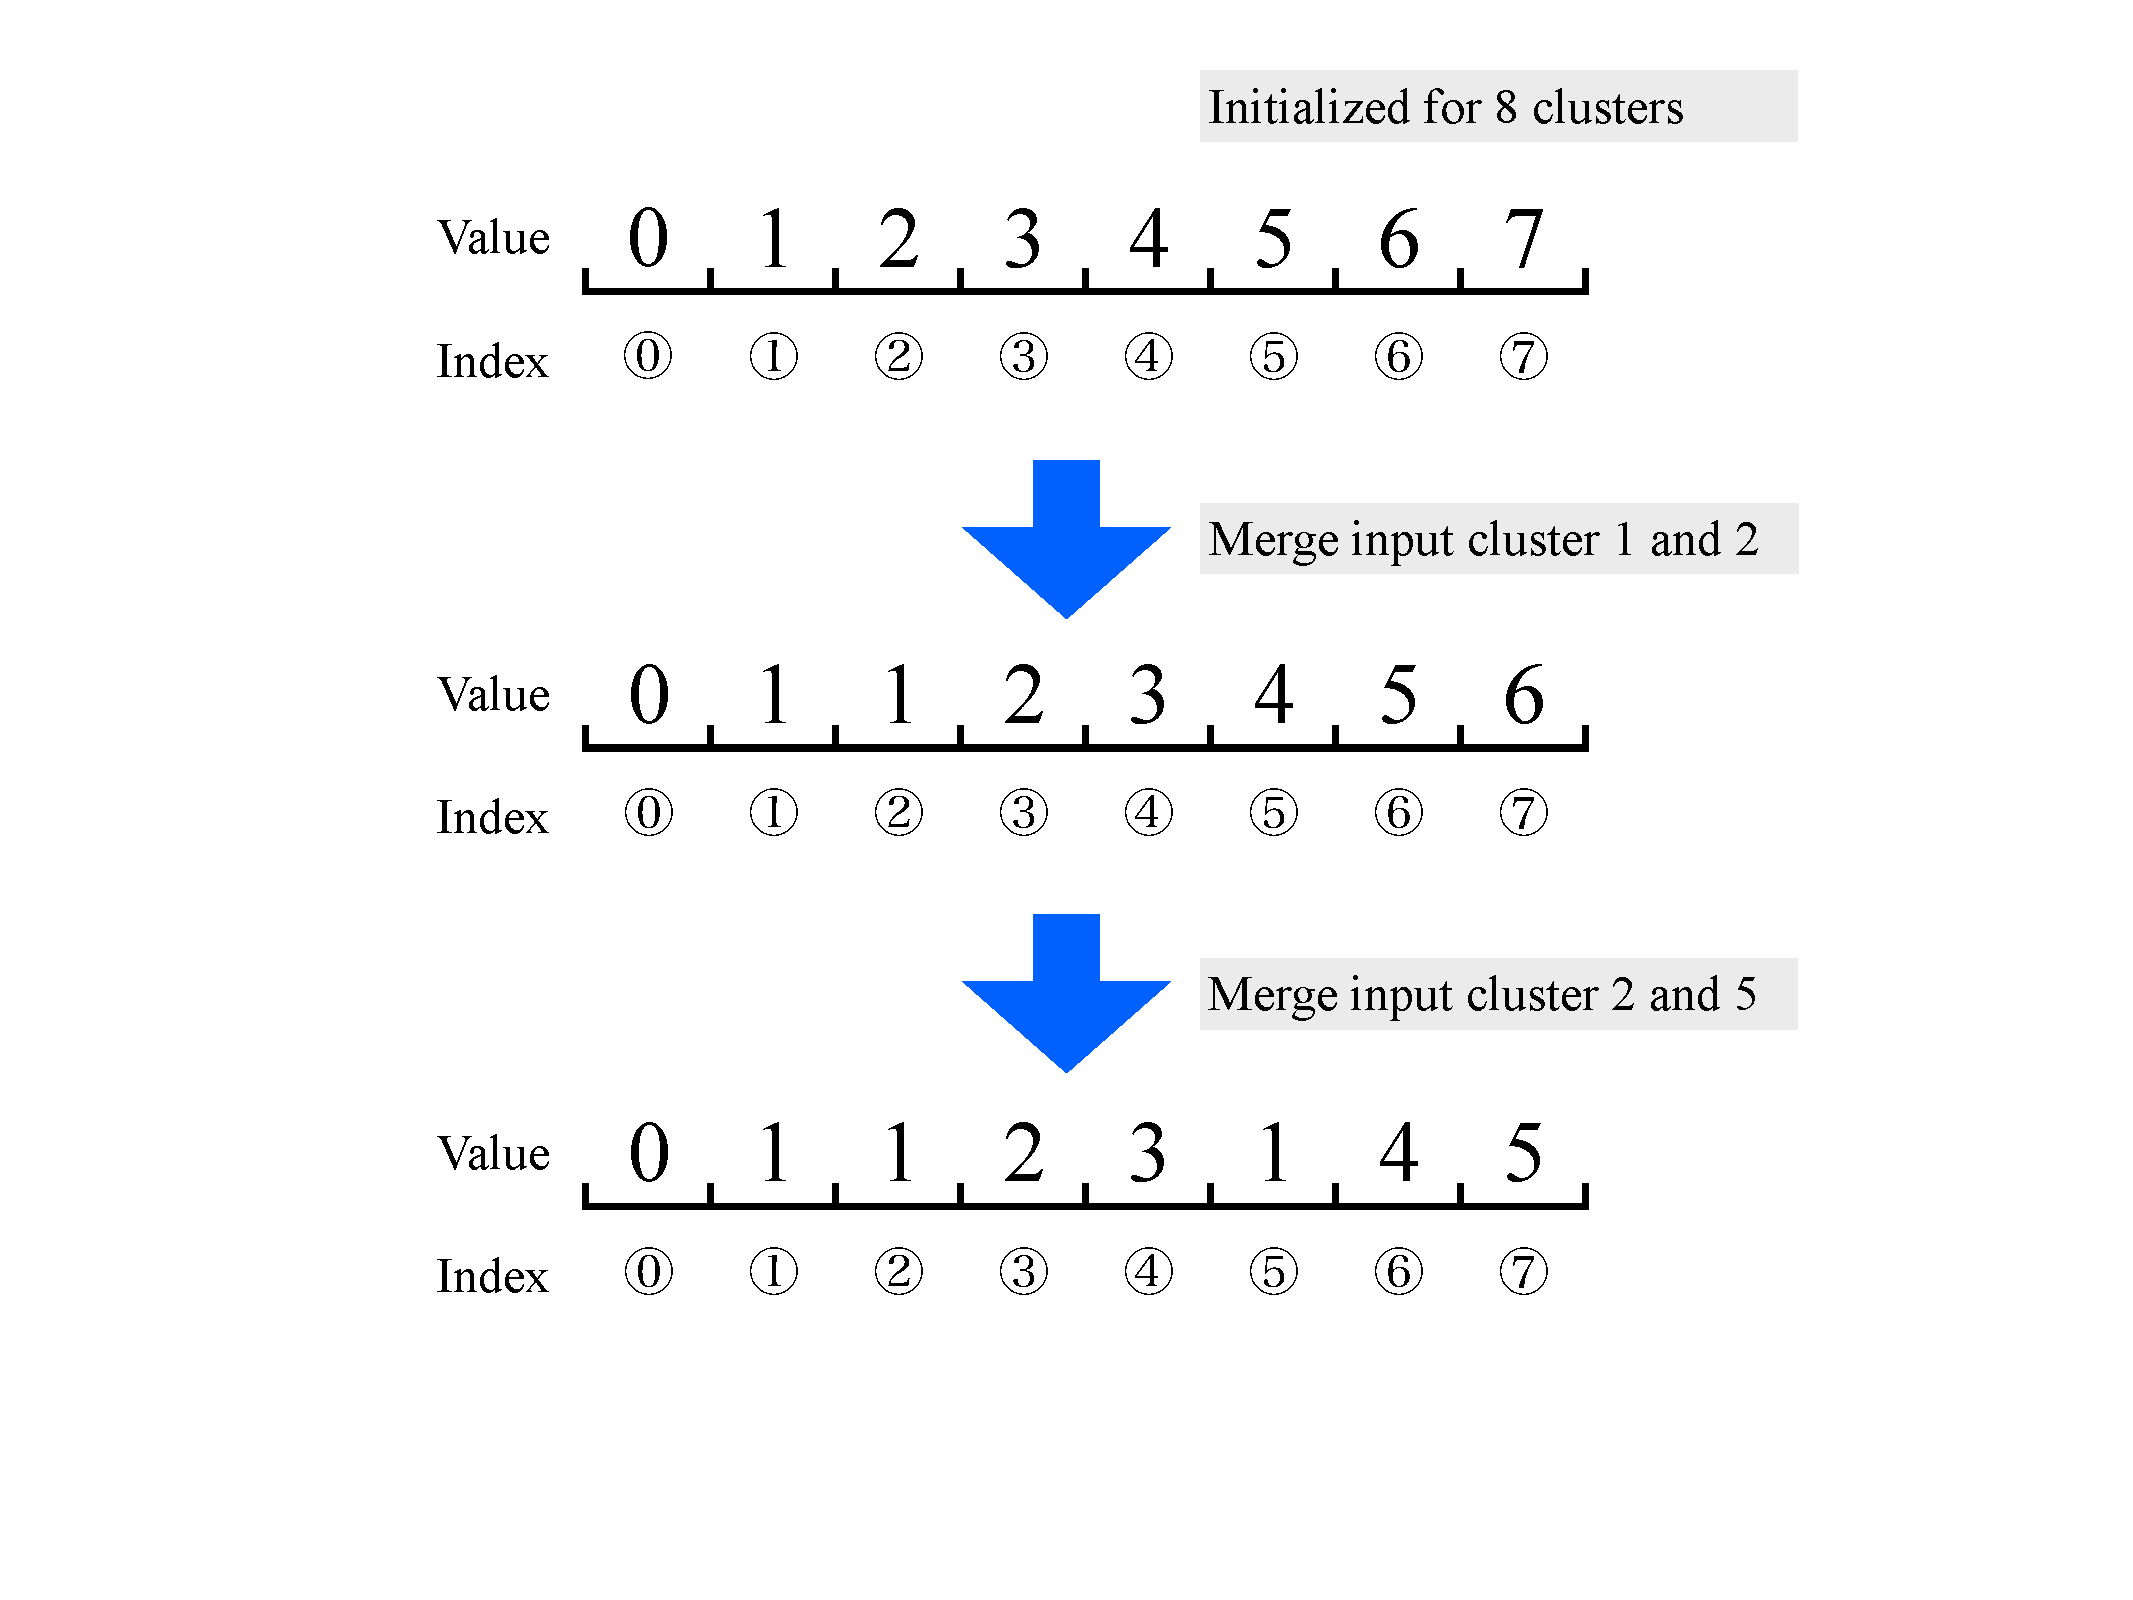
\includegraphics[width=14cm]{./src/Pictures/CBookKeeperExample.pdf}
\caption{Example diagram showing how {\cbkeeper} keeps track of input and output cluster IDs. It shows {\cbkeeper} vector index (input cluster ID) and stored values (output cluster ID) for 8 input clusters (top), and how the stored values change as merging takes place. The middle shows the result of merging input cluster 1 and 2, and the bottom is for further merging 2 and 5.}
\end{center}\end{figure}
When one finds 2 clusters to be merged together, (s)he can call {\cbkeeper} attribute function:
\begin{lstlisting}
        void CBookKeeper::Merge(unsigned short, unsigned short)
\end{lstlisting}
with corresponding clusters' IDs (i.e. index numbers). 
Figure \ref{sec:fmwk:base:cbk} shows how the process works for calling {\ttfamily CBookKeeper::Merge()} function twice with arguments (1,2) and (2,5).
As a result, unique output cluster IDs are reduced to 6 because 3 clusters are combined together.

You can see {\cbkeeper} instance allows to retrieve which output cluster (stored value) an input cluster (vector index) ended up with in an intuitive way: simply use {\ttfamily std::vector::at()} method.
However, to create an output cluster, it is probably easier to ask the other way around: given output cluster ID, which input cluster(s) does it contain?
{\cbkeeper} has a simple function to answer this question:
\begin{lstlisting}
        std::vector<std::vector<unsigned short> > GetResult() const 
\end{lstlisting}
which returns a vector with length same as number of output (i.e. merged) clusters.
The value of this vector is {\ttfamily std::vector<unsigned short>} to contain possibly multiple input cluster indexes.
For instance, the return from {\cbkeeper} shown in the bottom of Fig.\ref{sec:fmwk:base:cbk} would be a vector of length 6, and the index1 contains a vector of input cluster ID 1, 2, and 5 as they have been merged into output cluster ID = 1.
Equivalent result can be obtained also by using
\begin{lstlisting}
        void PassResult(std::vector<std::vector<unsigned short> >&)
\end{lstlisting}
if that suits one's usage. 

If you are interested in checking which input cluster(s) included in a particular output (merged) cluster, you can use:
\begin{lstlisting}
        std::vector<unsigned short> GetMergedSet(unsigned short)
\end{lstlisting}
which takes an output cluster index as an argument and returns a vector that contains a list of input clusters that consist the output.

\begin{figure}[ht]\begin{center}
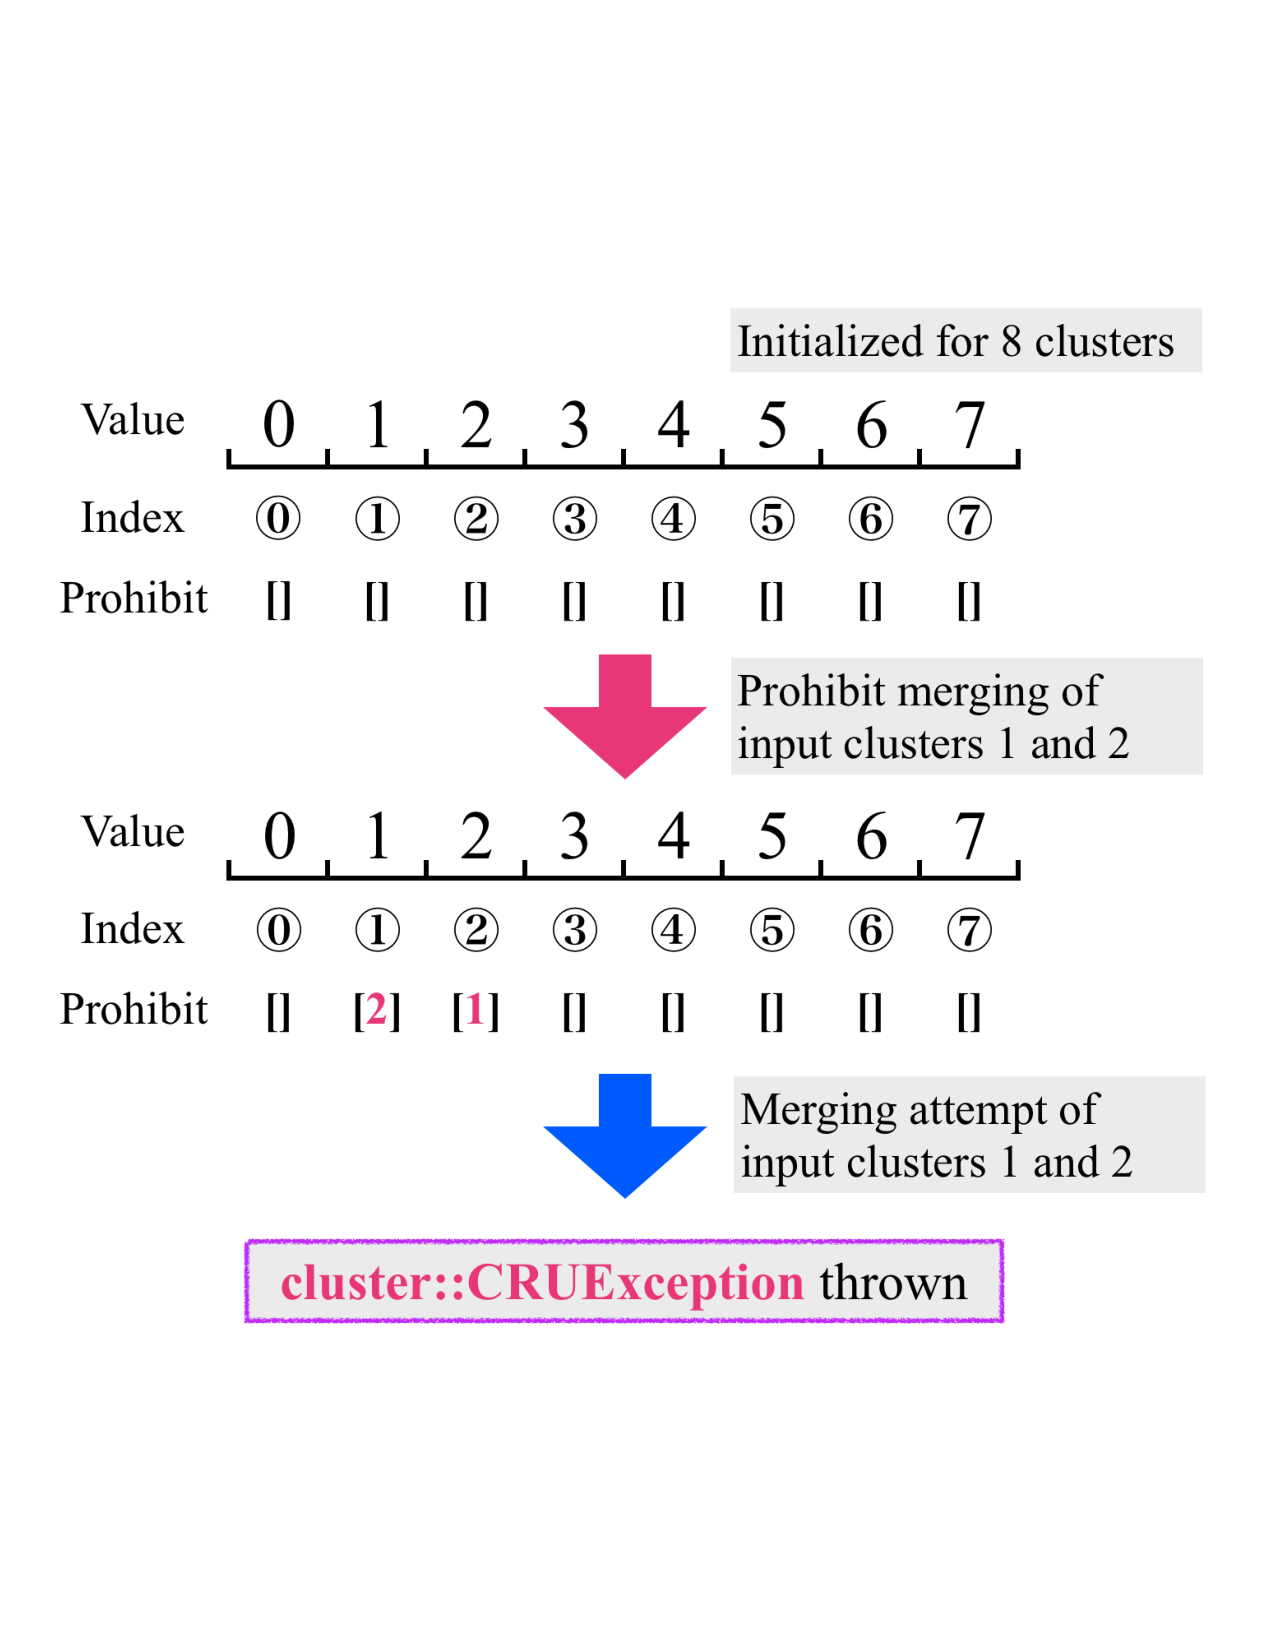
\includegraphics[width=8.3cm]{./src/Pictures/CBookKeeperProhibitExample2.pdf}
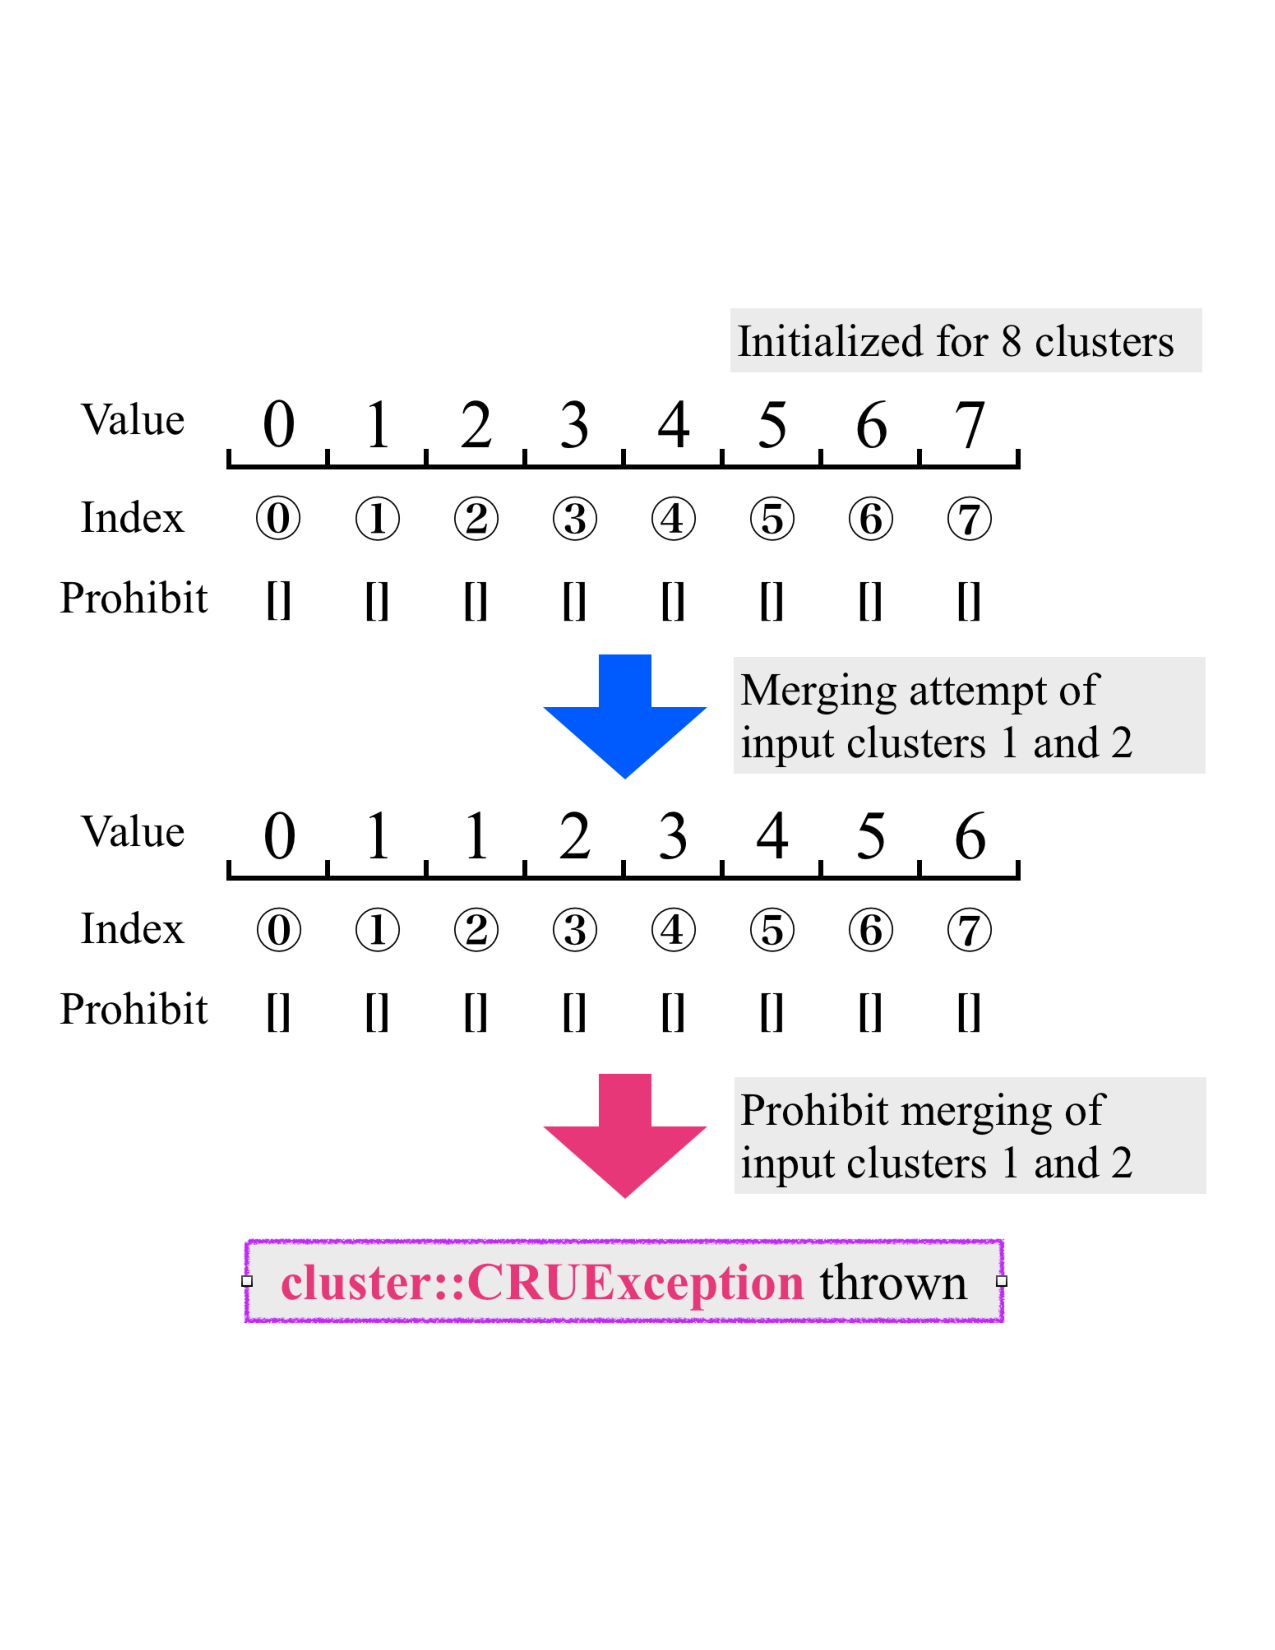
\includegraphics[width=8.3cm]{./src/Pictures/CBookKeeperProhibitExample1.pdf}
\caption{Example diagrams showing how {\cbkeeper} reacts to conflict {\ttfamily Merge()} and {\ttfamily ProhibitMerge()} function calls on the input cluster IDs. The left diagram shows {\crue} thrown due to calling {\ttfamily Merge()} on a cluster pair that is registered as merge-prohibit pair. The right diagram shows a result from calling {\ttfamily ProhibitMerge()} on a cluster pair that is already merged.}
\label{sec:fmwk:base:cbk_prohibit}
\end{center}\end{figure}

Finally, {\cmerge} can also prohibit merging of specific two cluster pair(s), and this is incoorporated by {\cbkeeper} as well.
This is, again, to support user to log merging in a mindless manner.
A user may specify specific 2 cluster pair should not be merged. 
Then (s)he can use the following function to register these 2 clusters for merge-prohibit list.
\begin{lstlisting}
        void ProhibitMerge(unsigned short, unsigned short)
\end{lstlisting}
The above function takes input cluster IDs (i.e. index numbers). 
Once 2 clusters are registered as merge-prohibit pair, attempting a function call {\ttfamily Merge()} will result in {\crue} thrown.
This is illustrated in the left of Fig.\ref{sec:fmwk:base:cbk_prohibit}.
Another possible case that results in {\crue} thrown would be calling {\ttfamily ProhibitMerge()} function on two input cluster IDs that are already merged. This is shown in the right hand side of Fig.\ref{sec:fmwk:base:cbk_prohibit}.

To avoid {\crue}, one should register all cluster pairs to prohibit-merge list before trying any merge attempt.
Upon attempting to call {\ttfamily Merge()}, then, one can use the function:
\begin{lstlisting}
        bool MergeAllowed(unsigned short, unsigned short)
\end{lstlisting}
to check if a cluster pair is registered to merge-prohibit list.
Calling this function prior to evaluation of merging (i.e. running some computation algorithm to decide whether to merge or not) may save some computation time and help the overall speed of the program (this is implemented in {\cmerge}).

\subsection{Algorithm Base: {\ttfamily CBoolAlgoBase}}
\label{sec:fmwk:base:cbalgo}
{\cbalgo} is a simple {\CPP} template class and also a base class for an algorithm used for cluster merging and matching by {\cmerge} and {\cmatch} application classes. In this and later sections, we use the term {\cmalgo} to refer to an algorithm class derived from {\cbalgo}.

\begin{figure}[ht]\begin{center}
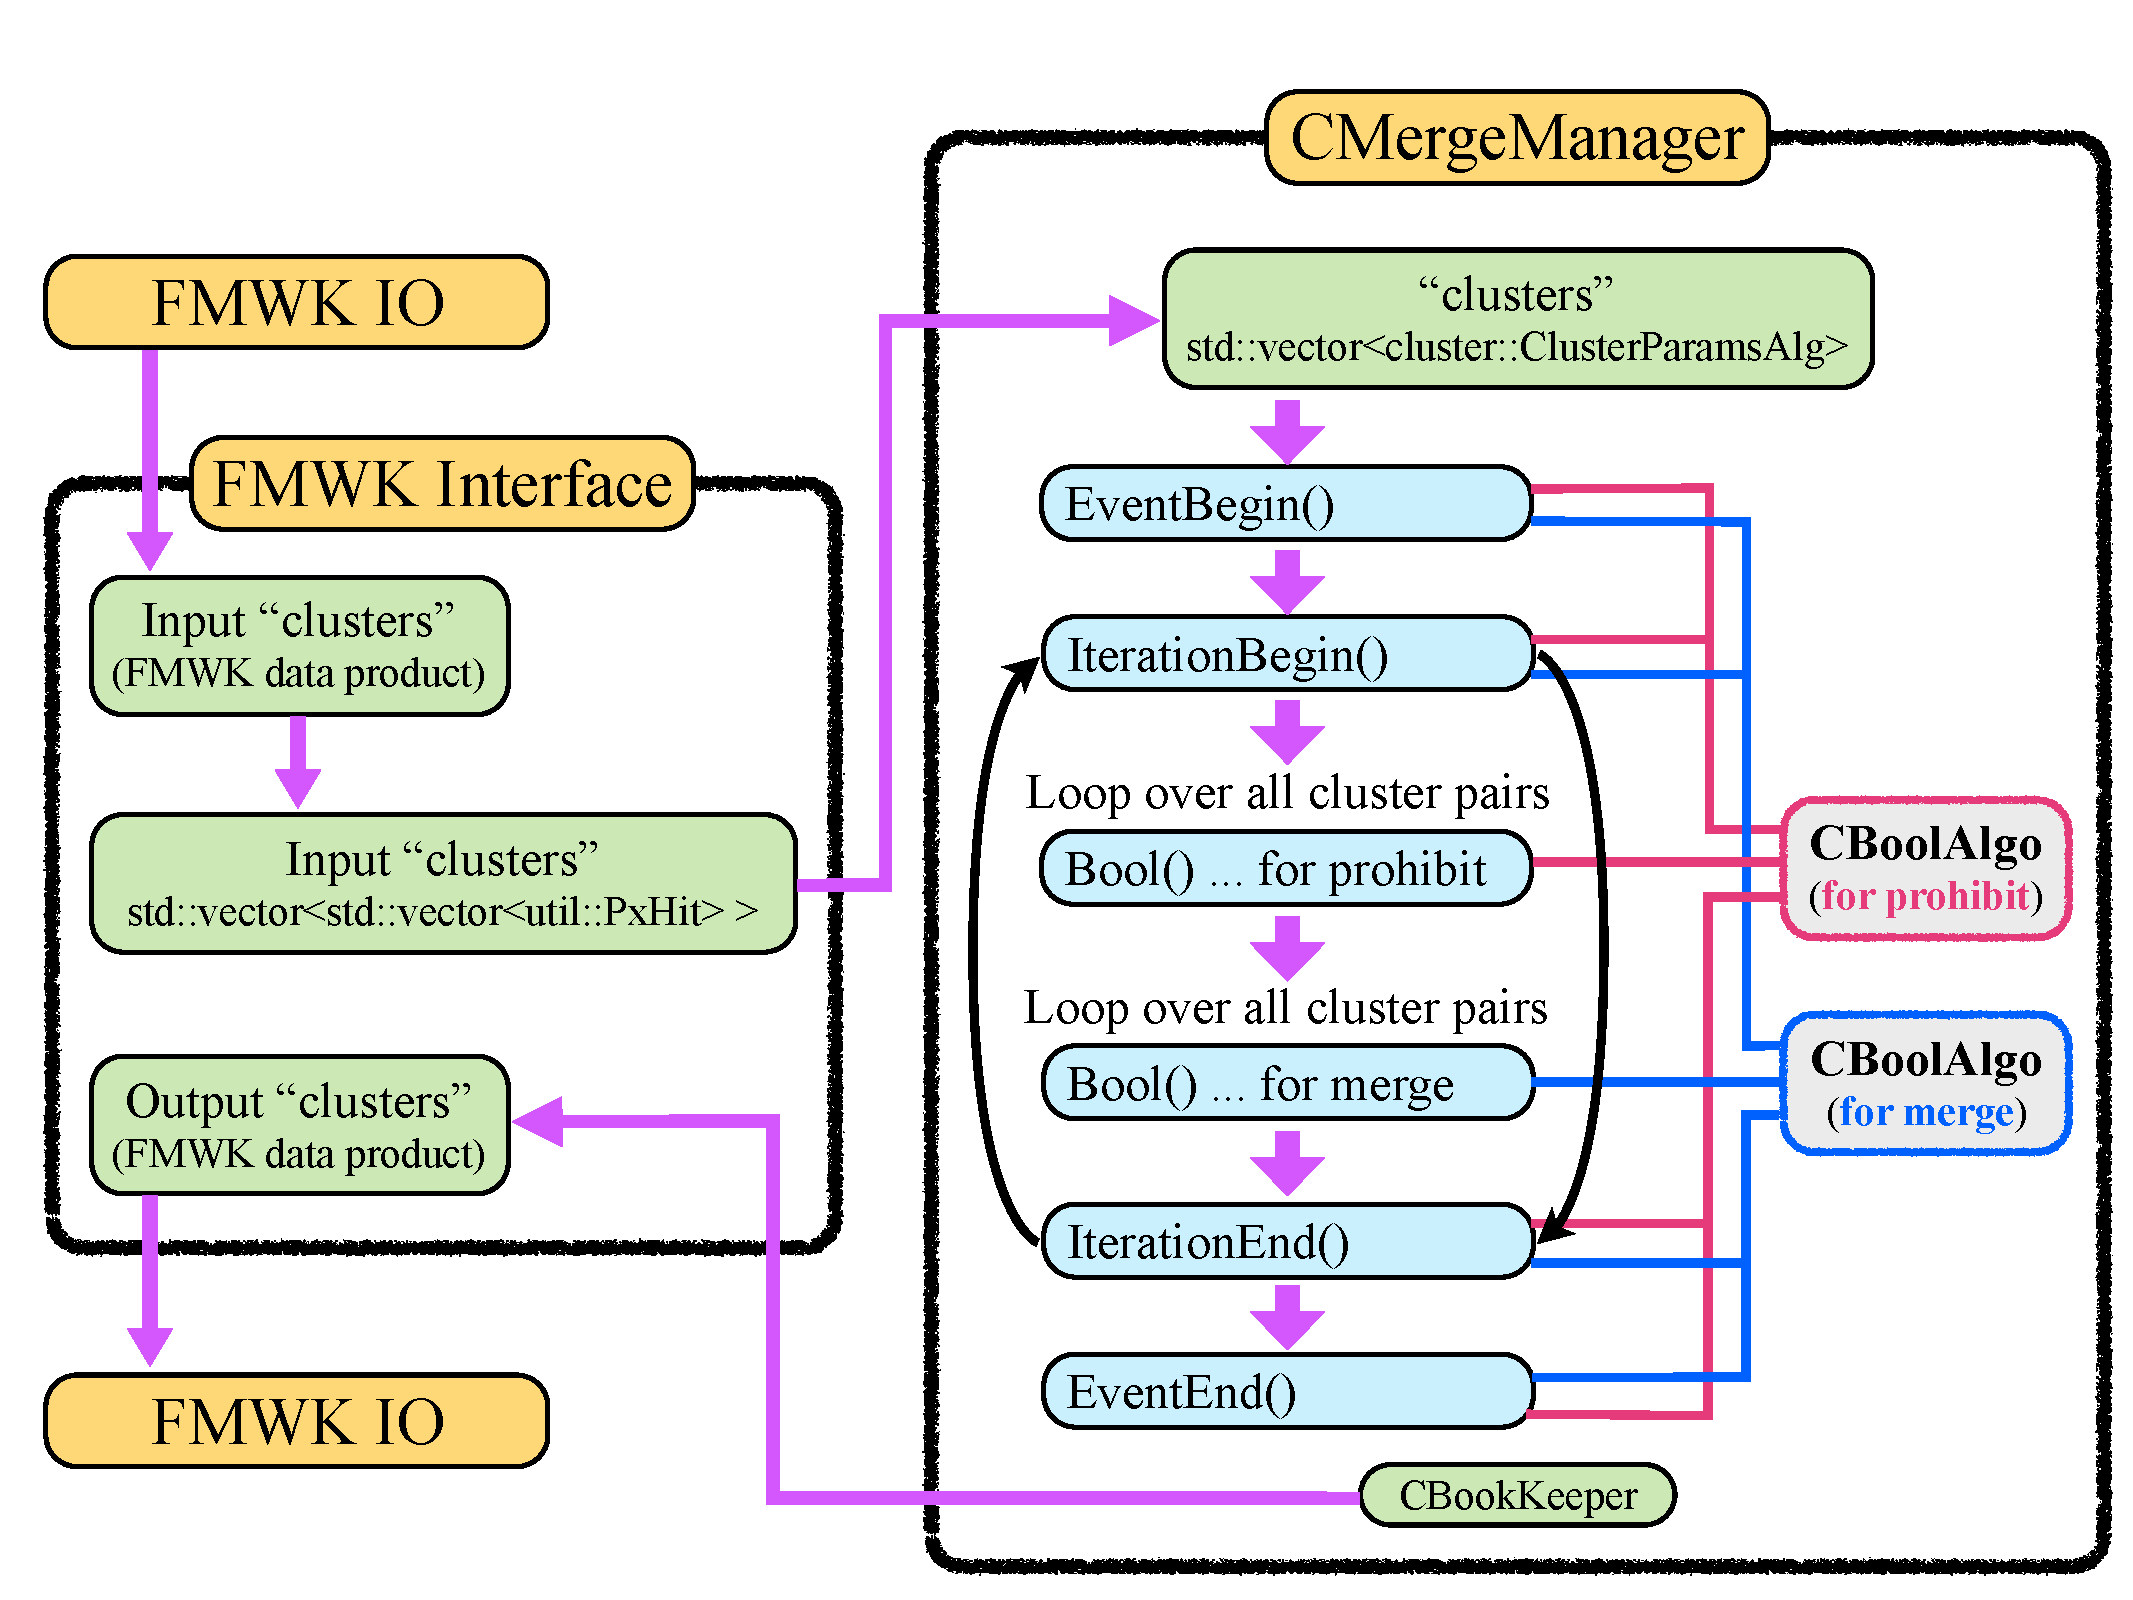
\includegraphics[width=13cm]{./src/Pictures/CMergeStream.pdf}
\caption{The data processing stream of {\cmerge} framework. The purple allow shows the ordered process flow. It requires an analysis framework interface to convert framework dependent cluster data produdct into a vector of {\pxhit} and hand over to {\cmerge} application. Internally {\cmerge} calls various members of {\cbalgo} instances: one for merging and another for prohibiting. There is a configuration in {\cmerge} to perform iterative approach, which repeats internal loop over possible cluster pairs until no more newly merged cluster is found in the output. The merged cluster groups (i.e. output) can be obtained through {\cbkeeper} instance by an analysis framework interface to form an appropriate output data product.}
\label{sec:fmwk:base:cmerge_stream}
\end{center}\end{figure}

The idea is very simple: given two clusters, it is expected to return a boolean for decision making from the following function.
\begin{lstlisting}
        virtual bool Bool(const cluster::ClusterParamsAlg &, const cluster::ClusterParamsAlg &)
\end{lstlisting}
As you can see, ``clusters'' are handed over in terms of {\cpan} instance.
In {\cmerge}, the cluster merging application class, for instance, this is used for making merge decision as well as prohibit-merge decision (i.e. {\cmerge} holds two {\cbalgo} inherit class instance, one for merging and another for prohibiting).
An algorithm developpers should write his/her own {\CPP} algorithm class by inheriting from {\cbalgo}.
In the derived class, the {\ttfamily Bool()} function implementation should be over-riden. 
There is a script to generate a template (i.e. empty) {\cbalgo} inherit class and everyone is encouraged to use it for starting a new algorithm class. These are:
\begin{itemize}
\item For {\larsoft}
\begin{itemize}
        \item[]{\ttfamily> python \$MRB\_TOP/srcs/larreco/RecoAlg/CMTool/mac/gen\_cmalgo.py NAME}
\end{itemize}
\item For {\larlight}
\begin{itemize}
        \item[]{\ttfamily> python \$MAKE\_TOP\_DIR/UserDev/ClusterStudy/bin/gen\_cmalgo NAME}
\end{itemize}
\end{itemize}
where {\ttfamily NAME} should be replaced by the new algorithm's name. 
Running above command results in creating {\ttfamily CMAlgoNAME.h} and {\ttfamily CMAlgoNAME.cxx} in the appropriate directory.
Then you can proceed to build following the framework's guidance.

As mentioned, {\cbalgo} is operated by {\cmerge} and {\cmatch} applications.
For a given event, there is an internal loop of calling {\ttfamily Bool()} on all possible cluster pairs.
To provide flexibility in algorithm design, those applications also call other functions of {\cbalgo} in its processing.

The following is a list of such {\cbalgo} functions.
\begin{itemize}

\item[]{\ttfamily virtual void EventBegin(const std::vector<cluster::ClusterParamsAlg>\&)}
  \begin{itemize}
    \item Called at the beginning of an event, prior to looping over cluster pairs. The provided function argument is a vector of {\cpan} for all clusters subject for merging. This is where computation that requires the whole, initial cluster sets should be done.
  \end{itemize}

\item[]{\ttfamily virtual void IterationBegin(const std::vector<cluster::ClusterParamsAlg>\&)}
  \begin{itemize}
    \item Called at the beginning of an each loop over cluster pairs. Note {\cmerge} and {\cmatch} can have multiple iteration of looping over possible cluster pairs if configured to do so. For instance {\cmerge} can take iterate over multiple loops till no more to-be-merged  cluster pair is found (see Sec.\ref{sec:fmwk:cmerge} and Sec.\ref{sec:fmwk:cmatch} for details). The argument of this function is an output cluster sets, in terms of {\cpan} instance, from the previous loop. In case of the 1st loop, the provided cluster sets is identical to those provided in the argument of {\ttfamily EventBegin()} function.
  \end{itemize}

\item[]{\ttfamily virtual void IterationEnd()}
  \begin{itemize}
    \item Called at the end of each merge or match attempt loop over all cluster pairs, to clean up or summarize information.
  \end{itemize}

\item[]{\ttfamily virtual void EventEnd()}
  \begin{itemize}
    \item Called at the end of each event, after all iterations over cluster pairs are done.
  \end{itemize}

\end{itemize}

Further, there are two functions that are not yet implemented in {\cmerge} nor {\cmatch} but ideas exist.
Your input on how these should be implemented is welcome and very much appreciated.
\begin{itemize}

\item[]{\ttfamily virtual void Reset()}
  \begin{itemize}
    \item Meant to clear some member variables. But one can do that within {\ttfamily IterationEnd()} and/or {\ttfamily EventEnd()}, so it is not clear where this should be called. Possibly at the end of the whole event processing.
  \end{itemize}

\item[]{\ttfamily virtual void Report()}
  \begin{itemize}
    \item Meant to support some standardized {\ttfamily std::cout} and {\ttfamily std::cerr} report from an algorithm instance. {\cmerge} and {\cmatch} have ability to control such text output for different levels, and there is a hope this {\ttfamily Report()} can be also included there.
  \end{itemize}

\end{itemize}

\paragraph{Tips for writing {\cmalgo}}
First of all, you are encouraged to use {\ttfamily gen\_cmalgo} script as described earlier.
Another thing to note is to reduce a dependency on analysis framework.
This makes it easier to port your code between different frameworks.

